\chapter{Educational Synergy in Teaching and Research}
\section*{Introduction}

This appendix outlines the dual role I embraced during my semester as both a Teaching Assistant (TA) in the course "SW2PLA: Practical Linear Algebra for Software Engineers" and doing research for my Bachelor's thesis. My unique position allowed me to bridge theoretical understanding and practical application, fostering an educational environment where concepts in linear algebra, that are taught in the SW2PLA course, were directly linked to research in Large Language Models (LLMs).

\section*{Dual Role and Synergistic Learning}

As a Teaching Assistant in the SW2PLA course, my responsibilities included assisting students with practical exercises, grading assignments, and engaging in discussions about linear algebra during lectures. These activities were aimed at deepening students' understanding of linear algebra's application in modern computational technologies, particularly within the realms of basic AI and and elementary machine learning.
Simultaneously, my bachelor's thesis focused on integrating linear algebra within the development and optimization of LLMs, specifically assessing the effectiveness of low-rank approximation by SVD of Facebook's BART-model's attention weight matrices. Which gave me a new perspective on the practical applications of linear algebra in AI research and a further understanding of the linear algebra concepts taught in the SW2PLA course.

\section*{Project Overview in SW2PLA}

The final project for the SW2PLA course required students to undertake a practical application of eigendecomposition or SVD. The project aimed to provide hands-on experience with linear algebra's potent applications, offering several avenues for exploration:

\begin{enumerate}
  \item \textbf{Recommender Systems}: Using SVD to predict user preferences based on past interactions.
  \item \textbf{PageRank Algorithm}: Implementing an eigenvector-based approach to rank web pages.
  \item \textbf{Image Compression}: Applying SVD to reduce the dimensionality of image data without losing significant information.
  \item \textbf{Fibonacci Algorithm} Using eigendecomposition to compute the Fibonnaci algorithm without recursion.
  \item \textbf{Eigenportfolios}: Employing eigendecomposition for optimized stock portfolio selection.
  \item \textbf{Facial Recognition}: Utilizing PCA (a form of eigendecomposition) to identify and classify facial features in images.
  \item \textbf{Open Project}: Any project idea involving Eigendecomposition or SVD. Whether it's applying these techniques to optimize algorithms, enhance data processing, or explore new applications, approaches or innovative use of linear algebra.
\end{enumerate}

\section*{Integration with Bachelor's Thesis}

During the course, I also had the opportunity to present the methodologies and intermediate findings of my bachelor's thesis to the class. This presentation served as a practical demonstration of how linear algebra is utilised within the development and optimization of LLMs—particularly through techniques like low-rank approximations and matrix factorizations—to enhance computational efficiency and model scalability. This further provided students with real-world applications of their theoretical studies.

\section*{Student Projects and Feedback}

The culmination of the course was the student presentations, where they demonstrated their projects' outcomes. This session provided an interactive platform for peer learning and feedback, where students could showcase their application of linear algebra in various projects. My presentation alongside the students' highlighted the reciprocal nature of teaching/learning and research.

\section*{External Presentation and Recognition}

In addition to sharing my findings within the SW2PLA course, I had the opportunity to present the methodologies and intermediate results of my bachelor's thesis at a poster competition held during the Center for Language Generation and AI (CLAI) workshop. This presentation allowed me to engage with a broader audience of experts and peers in the field, receiving valuable feedback that furthered my research endeavors.

The highlight of this event was the recognition of the work, as the 3rd place in the competition was secured. This achievement not only affirmed the quality and relevance of my research in the field of AI but also provided a platform to showcase the practical applications of linear algebra in optimizing Large Language Models. This external validation brought additional perspective to the educational content I was delivering in the SW2PLA course, enhancing the overall teaching and learning experience.
\begin{figure}[H]
    \centering
    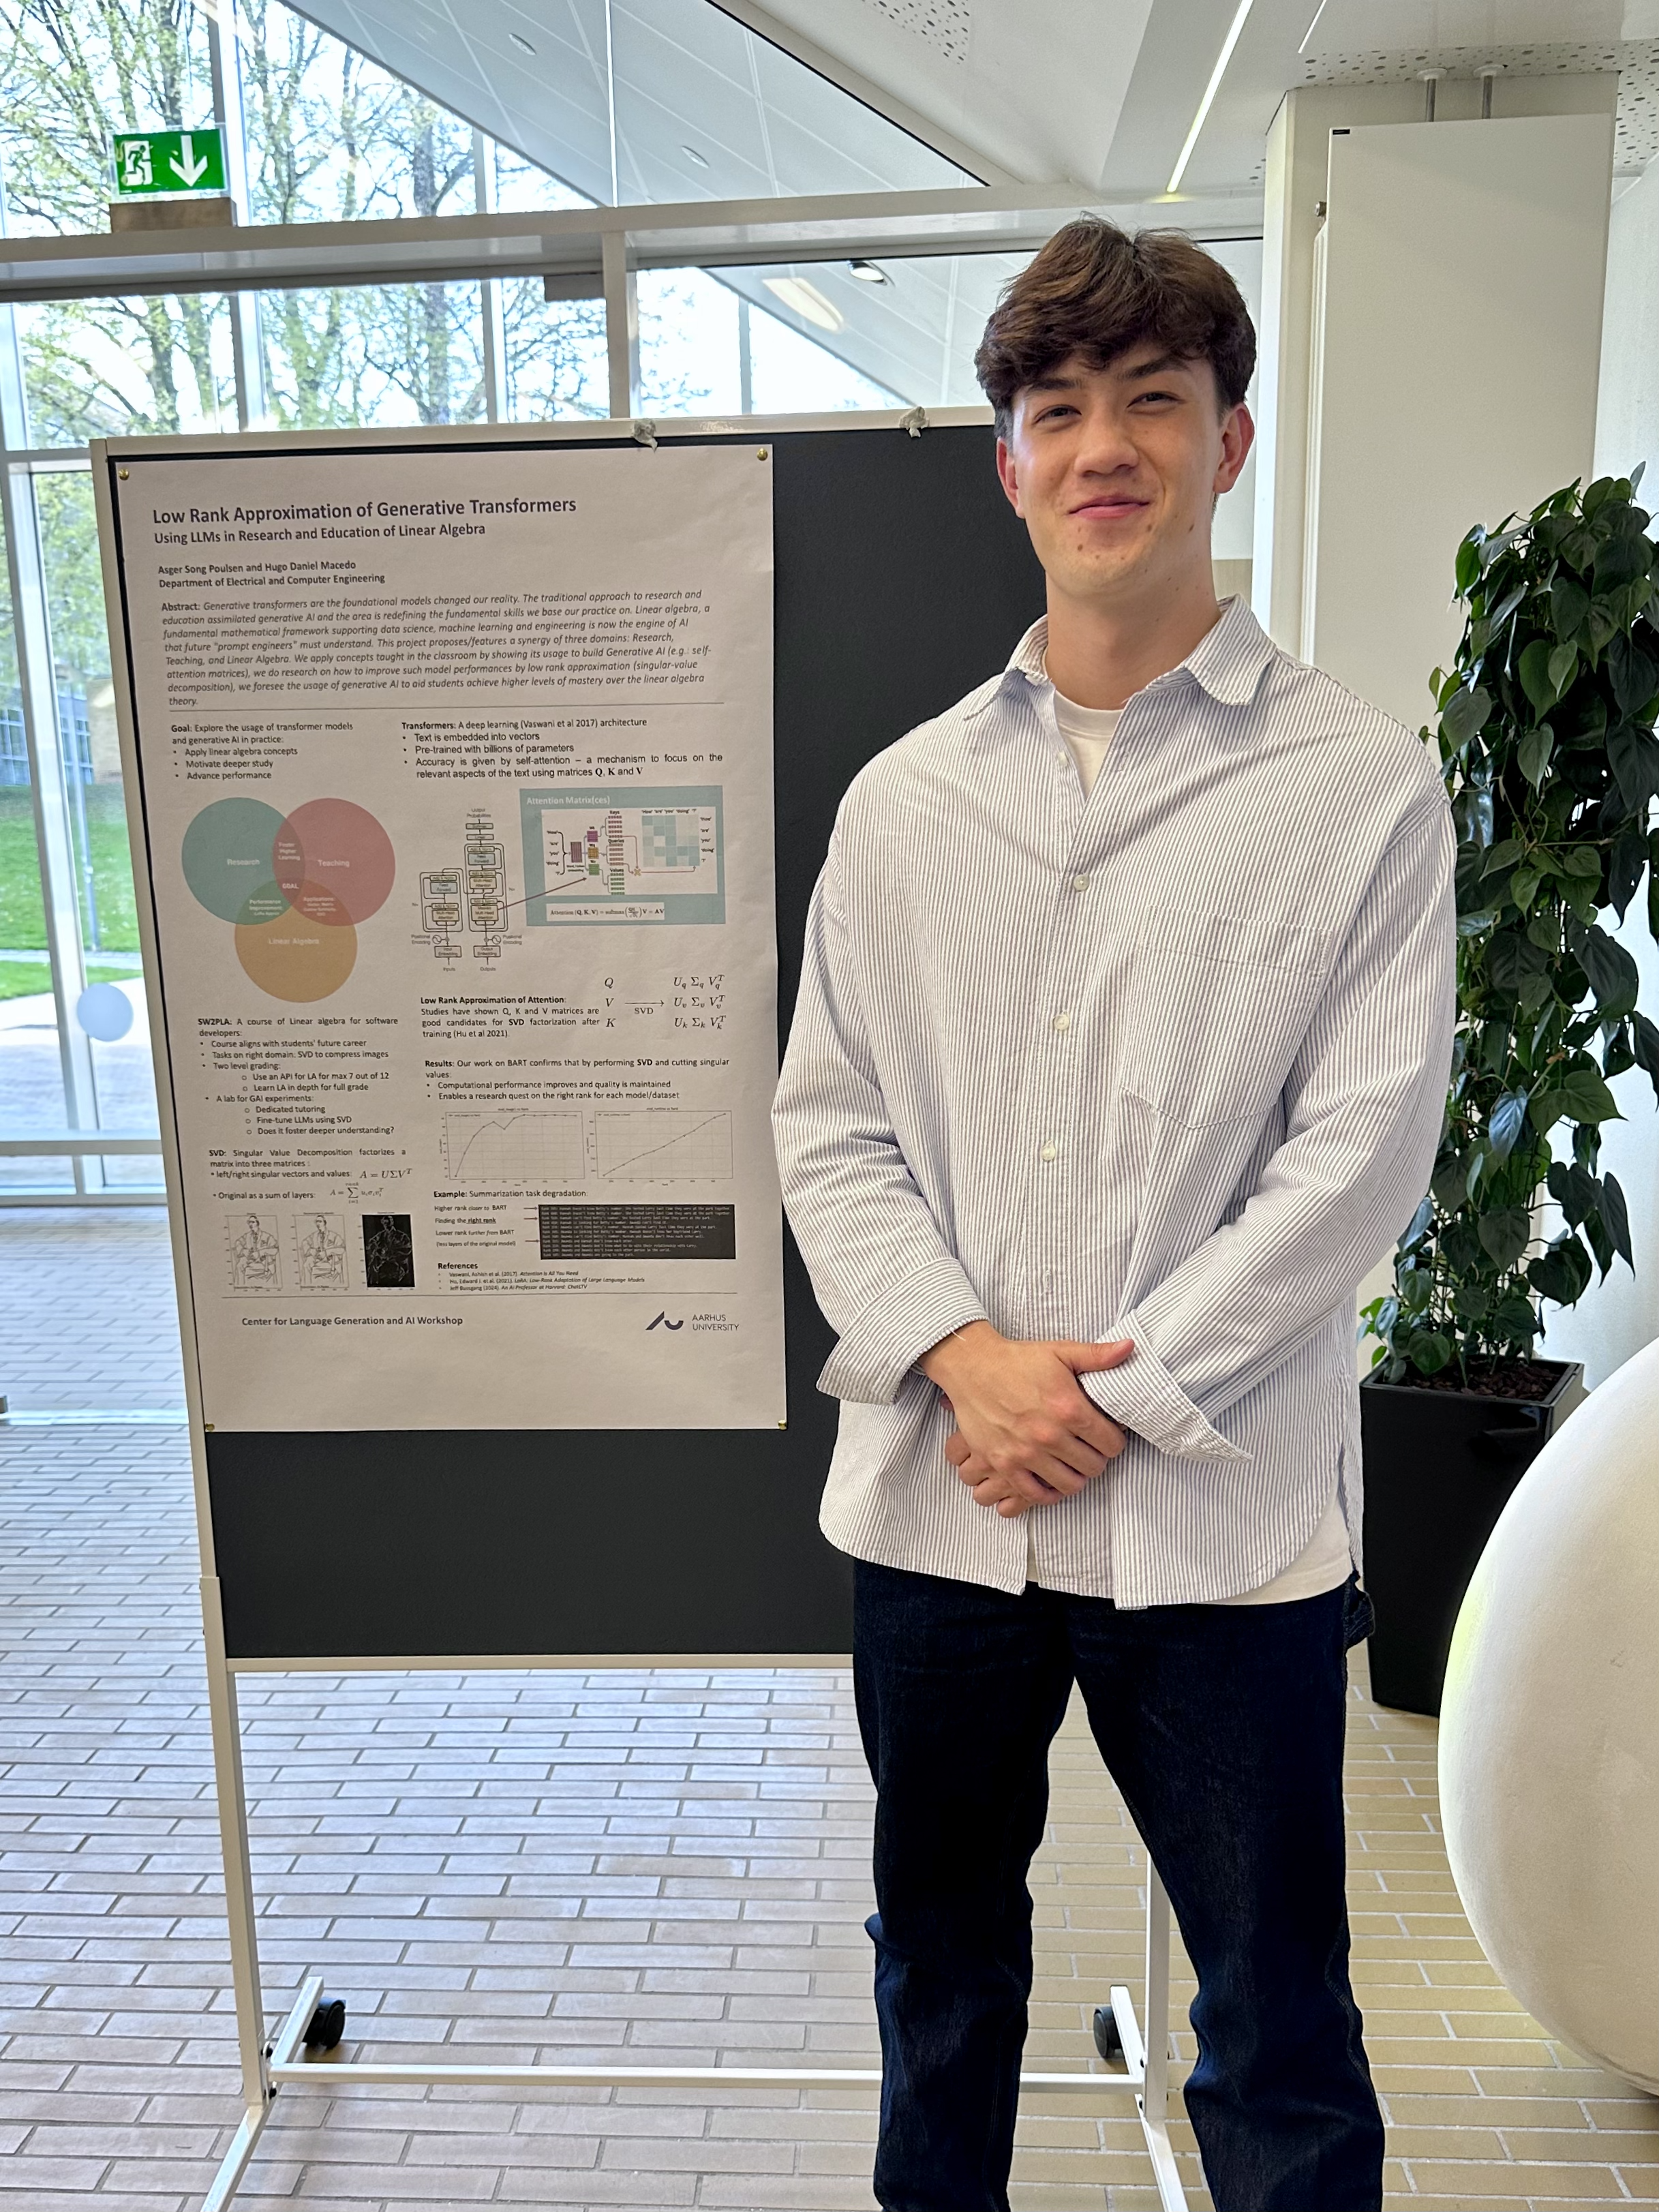
\includegraphics[width=0.6\textwidth]{figs/IMG_5113.png}
    \caption{3rd place in the CLAI Poster Competition}
    \label{fig:CLAI_Poster_Competition}
\end{figure}

It was an honor to represent the Department of Electrical and Computer Engineering (ECE) at such a forum. This accolade not only represents a personal achievement but also served as a good practice for me to present research findings to a broader audience, including students and faculty members from various disciplines.

\section*{Conclusion}

My involvement in the SW2PLA course as a TA, while simultaneously conducting research for my bachelor's thesis, created a rich educational synergy. This experience not only enhanced my understanding and teaching of linear algebra but also allowed me to directly apply and evaluate theoretical concepts in practical, research-based applications. It underscores the importance of an integrated approach in education, where teaching responsibilities and academic research complement and enrich each other, preparing students, and myself included, for future challenges in technology and engineering.